\documentclass[12pt, letterpaper]{report}
\usepackage[margin=1in]{geometry}
\usepackage[utf8]{inputenc}
\usepackage{graphicx}
\usepackage{float}
\usepackage{subfig}
\usepackage{indentfirst}
\graphicspath{ {./img/} }
\setlength\parindent{20pt}
\renewcommand\thesection{\Roman{section}.}


\title{CS1550 - Page Replacement Algorithm Analysis}
\author{Zachary M. Mattis}


\begin{document}
	
\maketitle


\section{Algorithm Analysis}

After implementing and analyzing several page replacement algorithms, including optimal, clock, first-in-first-out, and not recently used, the results of the algorithms are very clear when viewing the number of page faults plotted against the number of frames available in physical memory. Using 3 provided traces of memory accesses (bzip.trace, gcc.trace, swim.trace), the performance of each algorithm under different circumstances was analyzed. One thing to note is that the optimal algorithm cannot be practically implemented, as it involves predicting future memory accesses to determine the best frames to utilize resulting in the least amount of page faults. It was able to be implemented in this project due to the pre-parsing of the memory accesses for optimizations.

To determine the optimal performance of the NRU algorithm, the refresh rate parameter had to be analyzed. After N instructions have been processed, the NRU algorithm resets the referenced bit on all page table entries. Different values of the NRU refresh parameter were analyzed in Figure 1, and 50 selected to be used as the default amongst all other page faults comparison metrics. While the number of page faults continually decreases as the refresh rate goes up, this difference is nominal in comparison. 

Upon analyzing all four algorithms on the various traces as seen in Figures 2, 3, and 4, it is clear the optimal is be far the best page replacement algorithm. It provides the lowest amount of page faults which is the overall goal of a page replacement algorithm. However, as stated above, this implementation is unfeasible without knowledge of future memory accesses to predict behavior and minimize page faulting. As far as the other three algorithms, NRU seemed to be the worst implementation of all. It consistently provided a higher page faulting rate than clock and FIFO, and did not provide any clear benefits. The page faulting rate between clock and FIFO was generally close; however, clock provided better performance on the two last traces, as seen in Figures 3 and 4. This increase performance over FIFO is expected, as it reads the R bit of the page table to determine if the page has been referenced.

In conclusion, clock proves to be the superior paging algorithm, provided increase performance over both FIFO and NRU. As a practically implementable algorithm, it demonstrates its superiority as it has the lowest page faulting rate.


\section{Appendix}

\begin{figure}[H]
	\centering
	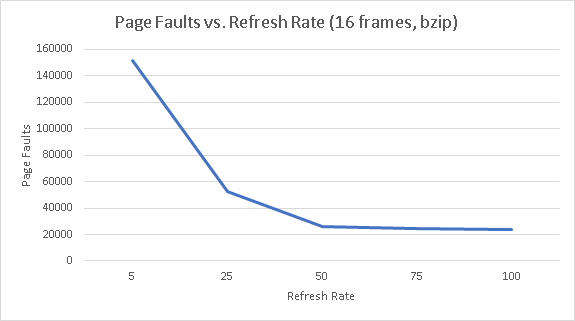
\includegraphics[width=0.7\columnwidth]{pagefault_refreshrate_bzip.png}
	\caption{Number of page faults vs. refresh rate– 16 frames, bzip.trace}
\end{figure}

\begin{figure}[H]
	\centering
	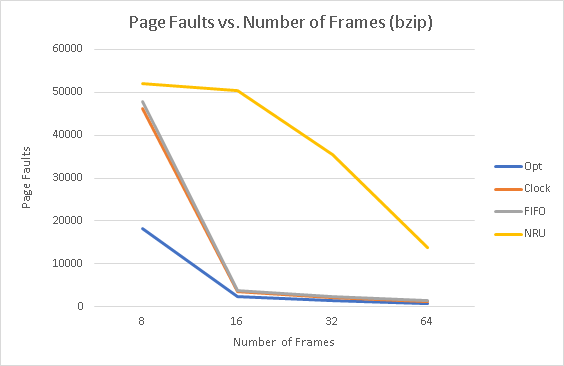
\includegraphics[width=0.7\columnwidth]{pagefault_numframes_bzip.png}
	\caption{Number of page faults per number of frames – bzip.trace}
\end{figure}

\begin{figure}[H]
	\centering
	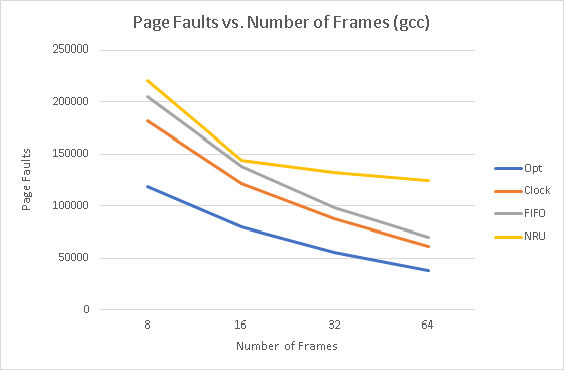
\includegraphics[width=0.7\columnwidth]{pagefault_numframes_gcc.png}
	\caption{Number of page faults per number of frames – gcc.trace}
\end{figure}

\begin{figure}[H]
	\centering
	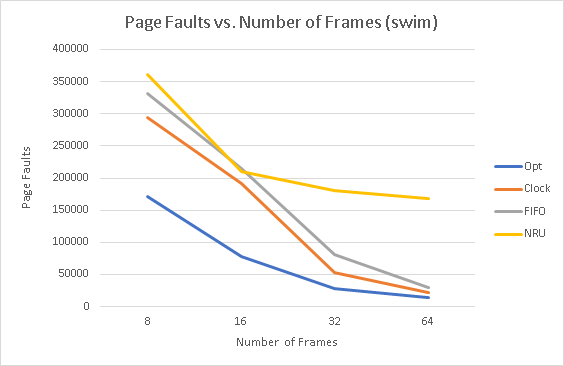
\includegraphics[width=0.7\columnwidth]{pagefault_numframes_swim.png}
	\caption{Number of page faults per number of frames – swim.trace}
\end{figure}


\end{document}